\documentclass[border=10pt]{standalone}
\usepackage[svgnames]{xcolor}
\usepackage{amsmath}
\usepackage{pgfplots}
\pgfplotsset{compat=newest}
\usepackage[sfdefault]{FiraSans}
\usepackage{FiraMono}
\renewcommand*\familydefault{\sfdefault}
\begin{document}
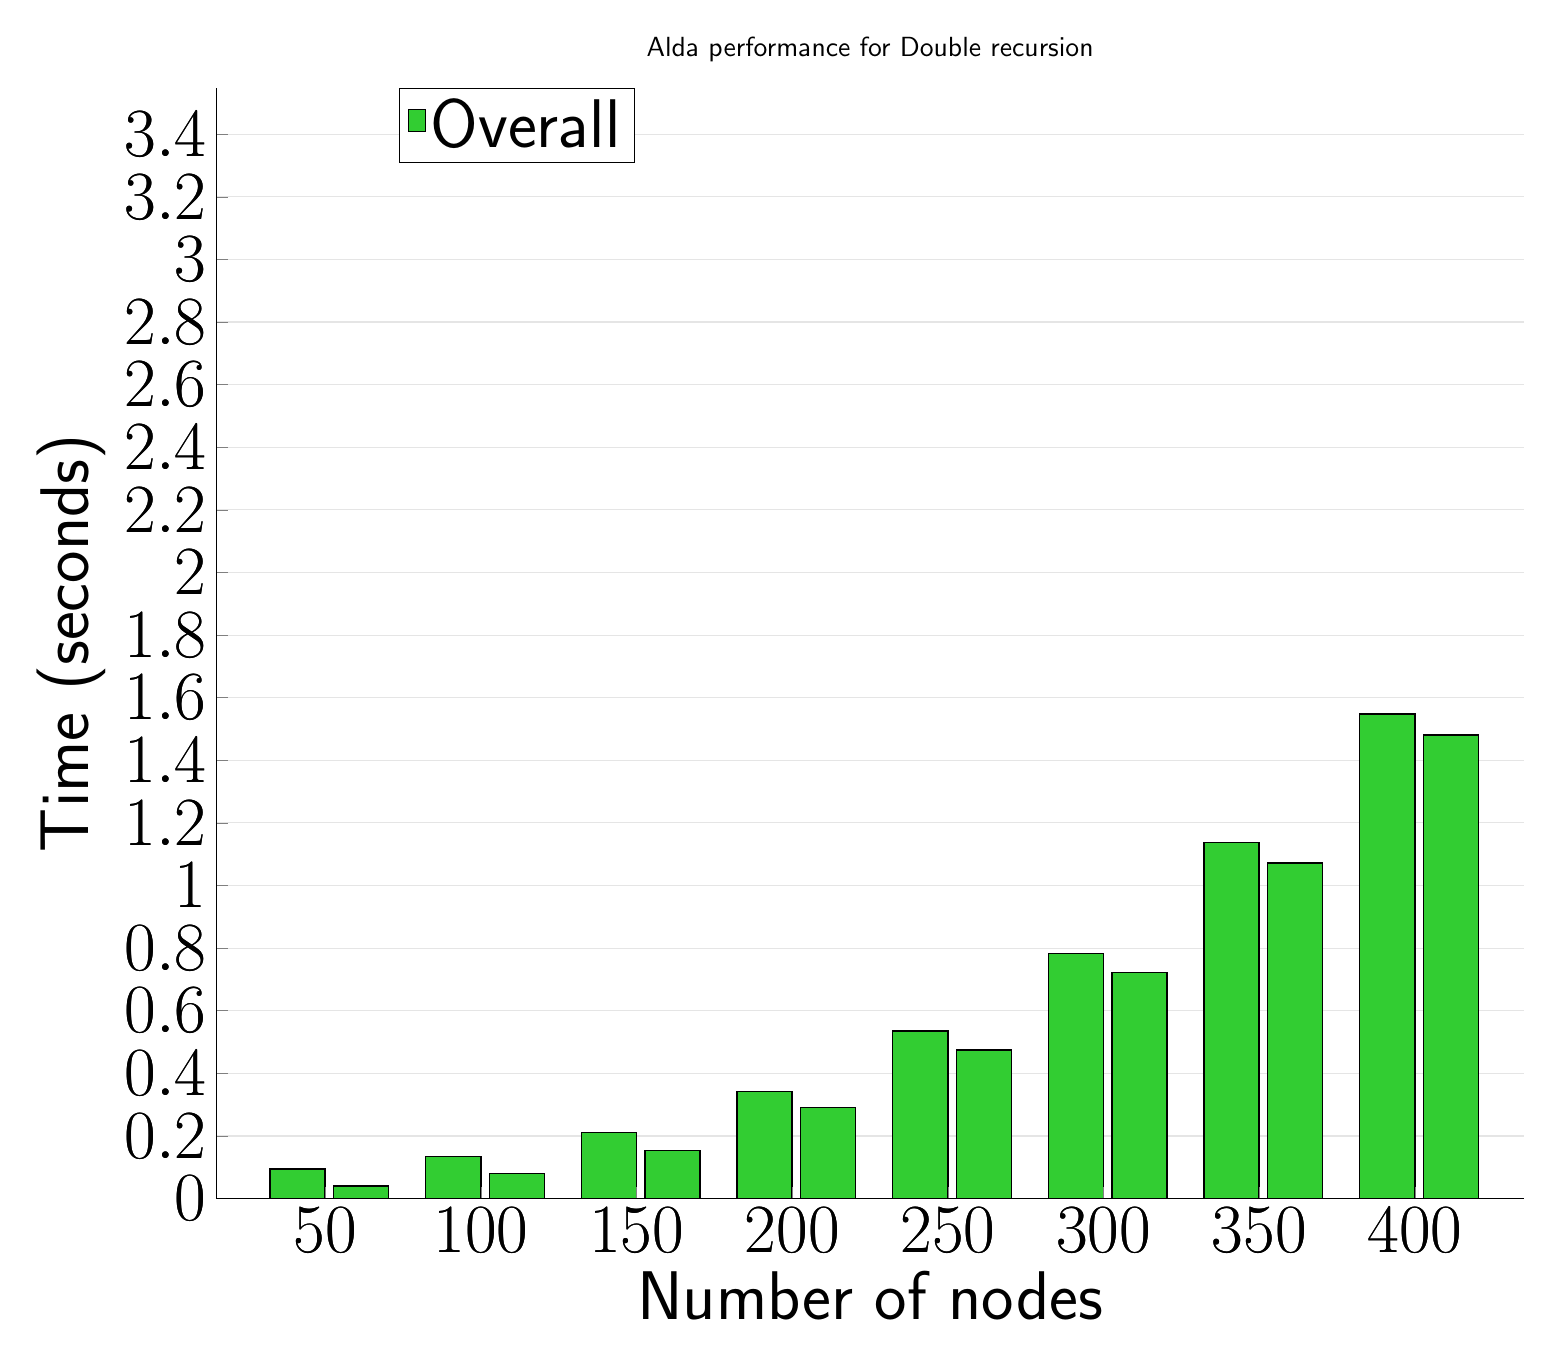
\begin{tikzpicture}
	\begin{axis}[
			ybar stacked,
			title={Alda performance for Double recursion},
			bar shift=-10pt,
			width=1.5\textwidth,
			bar width=0.7cm,
			ymajorgrids, tick align=inside,
			major grid style={draw=gray!20},
			xtick=data,
			ymin=0, ymax=3.5480000019073485,
			axis x line*=bottom,
			axis y line*=left,
			enlarge x limits=0.1,
			legend style={
					at={(0.23, 1)},
					anchor=north,
					legend columns=1,
					font=\Huge,
				},
			ylabel={Time (seconds)},
			xlabel={Number of nodes},
			label style={font=\Huge},
			tick label style={font=\Huge},
		]
		\addlegendimage{fill=LimeGreen, draw=black, line width=0.2pt}
		\addlegendentry{Overall}
		\addplot +[fill=LimeGreen, draw=black, line width=0.5pt] coordinates {
				(50, 0.09400000572204589)
				(100, 0.13399994373321533)
				(150, 0.21100001335144042)
				(200, 0.3419999837875366)
				(250, 0.5349999904632569)
				(300, 0.7829999923706055)
				(350, 1.137999987602234)
				(400, 1.5480000019073485)
			};
	\end{axis}
	\begin{axis}[
			ybar stacked,
			bar shift=13pt,
			width=1.5\textwidth,
			bar width=0.7cm,
			ymajorgrids, tick align=inside,
			major grid style={draw=none},
			xtick=data,
			ymin=0, ymax=3.5480000019073485,
			axis x line*=none,
			axis y line*=none,
			enlarge x limits=0.1,
			label style={font=\Huge},
			tick label style={font=\Huge},
		]
		\addplot +[fill=LimeGreen, draw=black, line width=0.5pt] coordinates {
				(50, 0.040000000000000015)
				(100, 0.07999999999999999)
				(150, 0.154)
				(200, 0.29000000000000004)
				(250, 0.4739999999999999)
				(300, 0.723)
				(350, 1.0720000000000003)
				(400, 1.481)
			};
	\end{axis}
\end{tikzpicture}

\end{document}
